\documentclass[12pt, a4paper]{article}
\usepackage{graphicx} 
\usepackage{listings}
\usepackage{xcolor} 
\usepackage[table]{xcolor} 
\usepackage{amsmath}
\usepackage{amssymb}
\usepackage{wrapfig}
\usepackage{parskip}
\usepackage{float}
\usepackage{hyperref}
\usepackage[utf8]{inputenc}
\usepackage[T1]{fontenc}
\usepackage{siunitx}
\sisetup{output-decimal-marker = {,}}
\usepackage[swedish]{babel}
\usepackage{array}
\usepackage{adjustbox}
\usepackage[margin=2.5 cm]{geometry}
\usepackage{appendix}
\usepackage{csquotes}
\usepackage{comment}
\usepackage{subcaption}
\usepackage[
    style=ieee,
    sorting=none
]{biblatex}
\usepackage{titling}
\usepackage{pdfpages}

\addbibresource{../references.bib}

\lstdefinestyle{mypython}{
    language=Python,
    basicstyle=\ttfamily\small,
    backgroundcolor=\color{gray!10},
    keywordstyle=\color{blue}\bfseries,
    %stringstyle=\color{orange!85!black},
    commentstyle=\color{green!50!black},
    numberstyle=\tiny,
    numbers=left,
    stepnumber=1,
    numbersep=8pt,
    showstringspaces=false,
    frame=single,
    breaklines=true,
    breakatwhitespace=true,
    tabsize=4,
    morekeywords={self},  % Lägg till fler Python-nyckelord om nödvändigt
    literate={ö}{{\"o}}1 {å}{{\aa}}1 {ä}{{\"a}}1 {\\}{{\textbackslash}}1 {±}{{$\pm$}}1
    {Å}{{\AA}}1,
    }
    
\begin{document}

\pagenumbering{arabic}
\thispagestyle{empty}
\begin{center}
{\huge\bf Förstudie - Fasta tillståndets fysik:\\}
\vspace{0.2cm}
{\Large\bf 
Bestämning av okänt grundämne med röntgendiffraktion samt analys av transmissionsspektrum hos kisel}
\end{center}
\vspace{0.2cm}
\begin{center}
Julius Berg (juliusbe), Benjamin Johansson (benjjoh), \par
Program: Teknisk fysik. \par
Kurs: TIF097 - Experimentell fysik 2.
\end{center}
\vspace{1.0cm}
\centerline{\bf Sammandrag}

Denna laboration syftar till att med hjälp av röntgendiffraktion identifiera ett okänt grundämne.
Dessutom studeras transmissionsspektrumet för kisel i våglängdsområdet 180 - 3000 nm.
Inledningsvis förbereddes ett prov av det okända grundämnet som placerades i en röntgendiffraktionskamera.
Därefter bestrålades provet under 40 minuter av en röntgenstråle.
Denna röntgenstråle diffrakterades och avbildades på en röntgenfilm som senare framkallades och avståndet mellan de diffrakterade reflexerna mättes.
Totalt genomfördes 3 mätningar och det okända grundämnet kunde konstateras ha en FCC-struktur med en gitterparameter på 3,61 Å.
Dessa värden stämmer väl överens med tabulerade värden för koppar, vilket grundämnet kunde identifieras som.
Därefter struderades transmissionsspektrum av kisel. 
Utifrån uppmätt transmissionsspektrum kunde kisel bekräftas ha ett indirekt bandgap på ca 1,19 eV
och fononabsorption i våglängdsområdet 5 - 20 µm.

\newpage
\tableofcontents
\newpage

\section{Inledning}
%Mer om optisk transmission
%Mer om kristallstrukturer?
%Varje kristallint material kan beskrivas med hjälp av en kristallstruktur och en eller flera gitterparametrar.  Ett ämnes kristallstruktur beskriver flera av ämnets egenskaper, exempelvis vilka reflexer som är tillåtna under diffraktion. Denna förstudie presenterar tillvägagångssättet att bestämma ett okänt grundämne med hjälp av Debye-Sherrer metoden. Dessutom kommer den optiska transmissionen av kisel att undersökas. -REWORK-


Varje kristallint material har en kristallstruktur som beskriver hur atomerna i kristallen är ordnade. 
Strukturen bestämmer också flera av kristallens egenskaper, exempelvis packningsdensitet eller vilka reflexer som är tillåtna under diffraktion\cite{Hofmann}. 
Denna förstudie presenterar en metod för att bestämma ett okänt grundämnes kristallstruktur och gitterparamater, med målet att specificera vilket grundämne som studeras.

Då ett ämne bestrålas av fotoner kan elektroner i ämnet exiteras genom att absorbera en foton med tillräckligt hög energi. 
Intensiteten på den strålning som passerar genom materialet minskar därmed. 
Genom att variera våglängden på den inkommande strålningen och mäta hur stor andel av intensiteten som passerar materialet kan ett transmissionsspektrum bildas\cite{Transmission}. 
Denna förstudie presenterar därmed också ett sätt att mäta transmissionsspektrumet för kisel.

\section{Teori}
% Kristallstrukturer generellt (kanske inledning)

Nedan readovisas för den här laborationen relavant teori.
Detta inkluderar grundämnens kristallstruktur, diffraktionsvillkor samt optisk transmission.
Även elektron- och fononexcitation diskuteras.

\subsection{Kristallstrukturern och diffraktion}

En kristall beskrivs matematiskt med hjälp av ett bravais-gitter, en oändlig uppsättning regelbundna punkter i rummet där varje gitterpunkt kan nås av en vektor, $R$, enligt
\begin{equation}
    \vec R = m\vec a_1 + n \vec a_2 + o \vec a_3,
\end{equation}
där $m, n, o$ är heltal, och $\vec a_1, \vec a_2, \vec a_3$ är tre linjärt oberoende gittervektorer. Gittervektorerna spänner dessutom upp kristallens enhetscell, som efter translation i gittervektorernas riktningar fyller hela rummet och ger en full beskrivning av kristallen.

Kristallen behöver däremot inte beskrivas i det reella rummet. Ett användbart verktyg är det reciproka rummet, som definieras av den reciproka gittervektorn, $\vec G = h\vec b_1+k\vec b_2+l\vec b_3$, där
\begin{equation}
    \vec b_1 = 2\pi \dfrac{\vec a_2 \times \vec a_3}{\vec a_1 \cdot(\vec a_2 \times \vec a_3)}, 
    \vec b_2 = 2\pi \dfrac{\vec a_3 \times \vec a_1}{\vec a_1 \cdot(\vec a_2 \times \vec a_3)},
    \vec b_3 = 2\pi \dfrac{\vec a_1 \times \vec a_2}{\vec a_1 \cdot(\vec a_2 \times \vec a_3)},
    \label{Eq: Reciproka vektorer}
\end{equation}
och $h,k,l$ är heltal. Från \ref{Eq: Reciproka vektorer} inses det att kortare längder i reella rummet blir längre längder i det reciproka, och omvänt\cite{Hofmann}.

Då en kristall bestrålas av exempelvis röntgenstrålning kommer strålningen reflekteras av på varandra följande atomplan i kristallen. 
Genom interferens mellan reflexerna uppstår ett diffraktionsmönster. För att erhålla konstruktiv interferens måste Braggs lag uppfyllas
\begin{equation}
    2d\sin(\theta) = n\lambda,
    \label{Eq: Braggs lag}
\end{equation}
där $d$ är avståndet mellan atomplanen, $\theta$ är den vinkel ingående och utgående stråla bildar med kristallplanen och $\lambda$ är strålningens våglängd. Det är däremot möjligt att reflexer som uppfyller Braggs lag inte ger konstruktiv interferens. Detta beror på ämnets kristallstruktur och dess strukturfaktor, $S_{hkl}$, som definieras enligt
\begin{equation}
    S_{hkl} = \sum_j f_j e^{2\pi i \vec G \cdot \vec r},
\end{equation}
där $\vec G$ är den reciproka gittervektorn, $\vec r$ är ortsvektorn för samtliga atomer i enhetscellen, och $f_j$ är respektive atoms formfaktor. Beroende på den kristallstruktur som bestrålas kommer specifika $hkl$ ge en strukturfaktor som är identisk lika med 0, vilket korresponderar till en förbjuden reflex. 

En metod för att deducera vilken kristallstruktur ett ämne består av är Debye-Sherrer-metoden, som grundar sig i att alla kristallstrukturer har olika tillåtna och förbjudna reflexer. Genom att låta ett fint pulveriserat prov bestrålas av röntgenstrålning erhålls med hjälp av en Debye-Sherrer-kamera ett cirkulärt diffraktionsmönster på en film, se figur \ref{fig:Debye_Scherrer_kamera}, och $\theta$ kan då beräknas enligt 
 \begin{equation}
     r = 2R\theta,
     \label{Eq:theta från cirkel}
 \end{equation}
där $r$ är radien på en godtycklig cirkel i diffraktionsmönstret och $R$ är kameraradien. Genom att studera vilka reflexer som är tillåtna respektive förbjudna kan en kristallstruktur specificeras. Genom omformulering av \ref{Eq: Braggs lag} fås
\begin{equation}
    d = \dfrac{\lambda}{2\sin(\theta)},
    \label{Eq: Bragg-omformulerad}
\end{equation}
där samtliga storheter överensstämmer med ekvation \ref{Eq: Braggs lag}. Däremot uttrycks $d$ annorlunda beroende på vilken kristallstruktur som undersöks. Exempelvis gäller för kubiska strukturer att
\begin{equation}
    d = \dfrac{a}{\sqrt{h^2+k^2+l^2}},
    \label{Eq: d-kubisk}
\end{equation}
där $a$ är gitterparametern. Genom insättning av \ref{Eq: d-kubisk} i \ref{Eq: Bragg-omformulerad} erhålls efter kvadrering och omformulering
\begin{equation}
    \sin^2(\theta) = \left(\dfrac{\lambda}{2a}\right)^2 (h^2+k^2+l^2).
    \label{Eq: Heltalsserie}
\end{equation}
Då $h,k,l$ är heltal kommer alltså $\sin^2(\theta)$ vara proportionerlig till en heltalsserie. 
Genom att beräkna $\theta$ för alla ringar på kamera-filmen och normalisera dessa erhålls alltså en heltalsserie, 
som kan matchas med kända serier för att utesluta vissa kristallstrukturer. 
Om strukturen inte skulle vara kubisk gäller däremot inte \ref{Eq: d-kubisk}, och \ref{Eq: Heltalsserie} antar en annan form. 
Däremot kan en liknande princip användas\cite{X-raylabbPM}.

Då kristallstrukturen är känd är även tillåtna och förbjudna reflexer kända. 
Genom att matcha varje ring till en uppsättning $hkl$ kan $a$ lösas ut och beräknas från \ref{Eq: Heltalsserie}.

\subsection{Optisk transmission}

Transmission, eller optisk transmission, $T$, beskriver hur mycket strålning som passerar genom ett givet material vid en specifik våglängd och definieras enligt
\begin{equation}
    T(\lambda) = \frac{I(\lambda)}{I_0},
\end{equation}
där $I(\lambda)$ är den transmitterade intensiteten och $I_0$ är intensiteten på den ingående strålen\cite{Transmission}.

Kisel har ett indirekt bandgap på $E_g = \SI{1,124}{eV}$\cite{physics_handbook}. 
Elektroner kan exciteras från valensbandet till ledningsbandet genom att absorbera fotoner med energi större än $E_g$. 
Detta medför en låg transmission. Motsatt, för fotoner vars energi är lägre än $E_g$ kommer transmittansen vara hög, då elektronerna inte kan exciteras till ledningsbandet. 
I området då fotonenergin är ungefär lika med $E_g$ erhålls en skarp övergång mellan områdena med låg och hög transmission.

Elektronexcitation är dock inte det enda sättet som en kristall kan interagera med fotoner.
Ett annat sätt är att fotonen kan excitera en eller flera fononer, som är kvantiserade vibrationer i gittret med en given energi\cite{Klemens_phonon}.
Fononens energi kan beskrivas som 
\begin{equation}
    E_f = \left(l + \frac{1}{2}\right)\hbar \omega(k)
    \label{eq:fonon_energi}
\end{equation}
där $l$ är ett positivt heltal, $\hbar$ är Plancks reducerade konstant, $\omega$ är vibrationens vinkelfrekvens och $k$ är vågtalet.
En foton kan alltså inducera en eller flera fononer med en lägre frekvens än fotonens egen.
Skulle detta ske kommer de resulterande fononerna ha energi enligt
\begin{equation}
    E_\gamma = E_i + E_j,
    \label{Eq:multifononabsorption}
\end{equation}
där $E_\gamma$ är fotonens energi och $E_i$ och $E_j$ är fononenergier.
Eftersom $\omega$ är en funktion av vågtalet $k$ och $k$ är kontinuerlig \cite{Hofmann} kommer detta ge upphov till ett band av fotonabsorption.

Fononer uppvisar olika frekvenser vid olika riktningar i det reciproka rkristallgittret.
Dessa olika riktningar ger upphov till olika grenar som kallas för dispersionsrelationer.
Kisel, som har en FCC-struktur med 2 atomer i basen, har 6 grenar.
Dessa grenar kallas för TA$_1$, TA$_2$ LA, LO, TO$_1$, TO$_2$ och hela dispersionsrelationen visas nedan i figur \ref{fig:dispersionsrelation_kisel}.

\begin{figure}[ht]
    \centering
    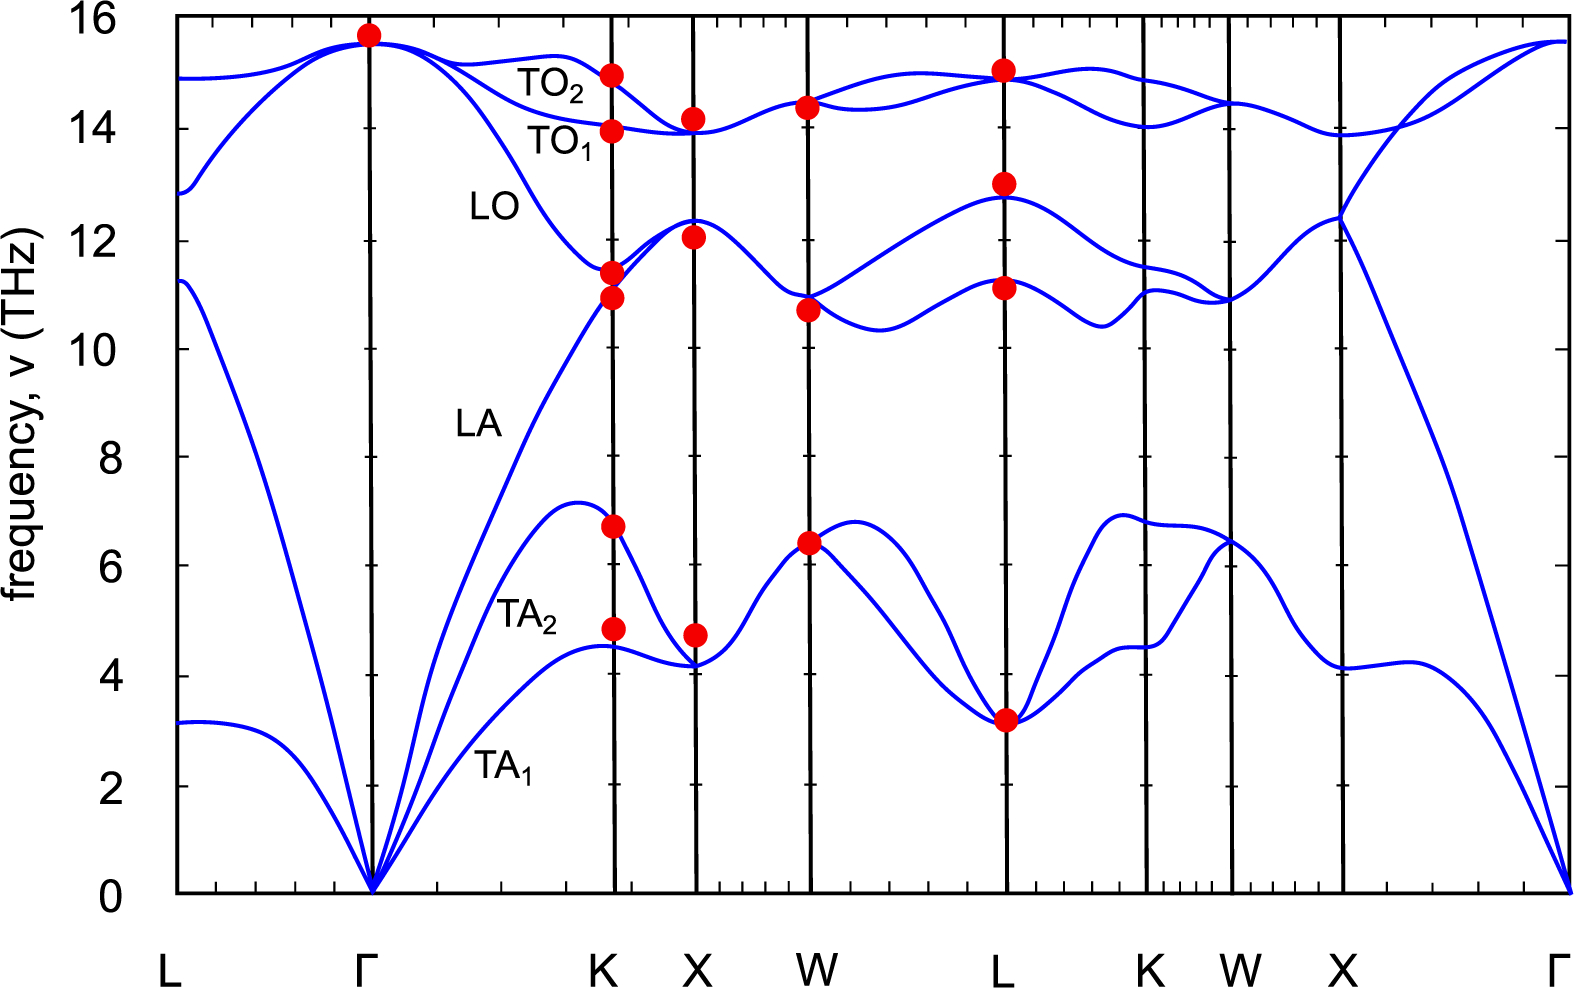
\includegraphics[width=0.7\textwidth]{Bilder/dispersionsrelation_kisel.jpg}
    \caption{\textit{Dispersionsrelation för kisel. Figuren visar 6 grenar längs med olika riktningar i det reciproka gittret.
    De röda punkterna är beräknade frekvenser vid de 5 första symmetripunkterna i det reciproka rummet och motsvarande värden redovisas i tabell \ref{tab:fononfrekvenser}.
    Figuren är tagen från \cite{phonons_silicon}.}}
    \label{fig:dispersionsrelation_kisel}
\end{figure}

De röda punkterna i figuren är beräknade vibrationsfrekvenser för de olika grenarna vid de 5 första symmetripunkterna i gittret.
Deras värden redovisas nedan i tabell \ref{tab:fononfrekvenser}. Värdena i tabellen är tagna från \cite{phonons_silicon}.
\begin{table}[H]
    \centering
    \renewcommand{\arraystretch}{1.2}
    \setlength{\tabcolsep}{3pt}
    \caption{\textit{Fononfrekvenser för olika dispersionsgrenar i symmetripunkter för kisel.
    Dessa värden motsvara de röda punkter som markerats i figur \ref{fig:dispersionsrelation_kisel}.
    Alla värden anges i THz.}}
    \begin{tabular}{|c|c|c|c|c|c|c|}
    \hline
    \rowcolor{lightgray} Symmetripunkt& TA$_1$ [THz] &TA$_2$ [THz]&LA [THz]&LO [THz]&TO$_1$ [THz]&TO$_2$ [THz]\\
    \hline
        $\Gamma$ & 0    & 0    & 0    & {}     & 15,63 & 15,63 \\
        X        & 4,71 & {}   & {}   & 11,98  & {}    & 14,09 \\
        L        & 3,14 & {}   & 11,05& 12,93  & {}    & 14,99 \\
        W        & 6,39 & {}   & {}   & 10,63  & {}    & 14,33 \\
        K        & 4,82 & 6,70 & 10,88& 11,30  & 13,90 & 14,91 \\
    \hline
    \end{tabular}
    \label{tab:fononfrekvenser}
\end{table}
% \begin{table}
% \centering
% \begin{tabular}{|c|c|c|c|c|}
% \hline
% \rowcolor{lightgray}
% Kristallstruktur & $1/d^2$    \\ \hline
% Kubisk & $\dfrac{h^2+k^2+l^2}{a^2}$ \\ \hline
% Tetragonal  & $\dfrac{h^2+k^2}{a^2} + \dfrac{l^2}{c^2}$ \\ \hline
% Hexagonal & $\dfrac 4 3 \dfrac{h^2+hk+k^2}{a^2} + \dfrac{l^2}{c^2}$ \\ \hline
% \end{tabular}
% \end{table}



% Exempelvis gäller för kubiska gitter


% där $a$ är gitterparametern och $\theta, \lambda, h,k,l$ överensstämmer med ekvation \ref{Eq: Braggs lag}. Då $a,\lambda$ är konstanter och $h,k,l$ är heltal är alltså $\sin^2(\theta)$ proportionerlig mot en heltalsserie
% \begin{equation}
%     \sin^2(\theta) \propto h^2+k^2+l^2.
% \end{equation}
% Genom att beräkna $\theta$ för alla ringar på filmen och normalisera dessa erhålls alltså en heltalsserie, som kan matchas med kända serier för att utesluta vissa kristallstrukturer. 
% %Optisk transmission


\section{Metod}
Nedan följer en beskrivning av den försöksuppställning som användes under laborationen.

\subsection{Försöksuppställning}
För att bestämma det okända grundämnet användes en Debye-Scherrer-kamera av modell 807 från företaget HUBER. 
För att generera en bild av diffraktionsmönstret så sprids diffraktionsstrålarna inuti kameran på insidan av en cylinder, på vilken en röntgenfilm monterades. 
Då Debye-Scherrer-metoden kräver att ett prov bestrålas med röntgenstrålning används även en röntgengenerator, 
i det här fallet en Siemens Kristalloflex 710. 
En schematisk bild över försöksuppställningen visas i figur \ref{fig:Debye_Scherrer_kamera}, där man kan se en infallande röntgenstråle träffa ett prov placerat i mitten. 
Diffraktionsstrålarna avbildas därefter på röntgenfilmen.

\begin{figure}[H]
    \centering
    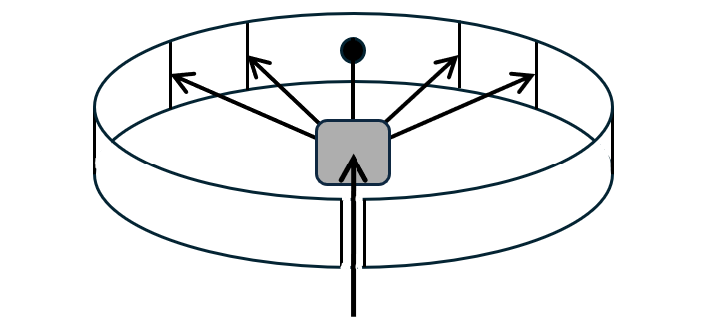
\includegraphics[width=0.8\linewidth]{../Förstudie/Bilder/Debye.Scherrer_kamera.png}
    \caption{\textit{Schematisk bild över en Debye-Scherrer-kamera. En infallande röntgenstråle träffar ett prov placerat i mitten. Provets kristallstruktur ger upphov till diffrakterande strålar som avbildar insidan av en cylinder, på vilken en röntgenfilm är placerad. Denna röntgenfilm kan efteråt framkallas och avstånden mellan de diffrakterande strålarna mätas.}}
    \label{fig:Debye_Scherrer_kamera}
\end{figure}

För att bestämma transmissionsspektrumet av kisel används ett färdigt kiselprov, en spektrofotometer av modell Cary 5000 och en spektrofotometer av modell Perkin Elmer 1725. 
Ett kiselprov placerades i mitten av en hållare som sedan placerades i spektrofotometern.
Figur \ref{fig:prov_i_perkin_elmer} visar kiselprovet placerat inuti Perkin-Elmer-spektrofotometern.
\begin{figure}[ht]
    \centering
    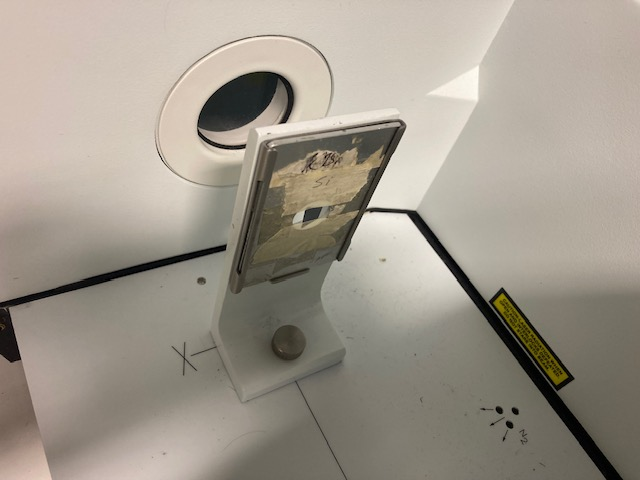
\includegraphics[width=0.5\textwidth]{Bilder/prov_i_perkin_elmer_closeup.jpg}
    \caption{\textit{Kiselprov placerat inuti en spektrofotometer av modell Perkin Elmer 1725.}}
    \label{fig:prov_i_perkin_elmer}
\end{figure}

Samma prov placerades därefter inuti Cary 5000-spektrofotometern.
\subsection{Genomförande}

% Inledningsvis bestäms det okända grundämnet med hjälp av Debye-Scherrermetoden. Provet prepareras och monteras inuti Debye-Scherrerkameran. 
% Därefter monteras röntgenfilm på insidan av kamerans mottagarcylinder. Provet bestrålas därefter med röntgenstrålning under 30 minuter för att 
% generera tillräckligt god upplösning på filmen för att analys skall kunna genomföras. Avslutnings framkallas filmen och avståndet mellan reflexerna mäts. 
% Avstånden kan därefter användas för att bestämma Braggvinkeln $\theta$, vilken tillsammans med ekvation \eqref{Eq: Heltalsserie} används för att bestämma 
% grundämnets kristallstruktur och gitterparameter.

% För att bestämma transmissionsspektrum av kisel placeras det färdiga kiselprovet i CARY 500-spektrofotometern och transmissionsspektrumet bestäms. 
% Därefter genomförs samma procedur med samma prov i Perkin Elmer 1725 spektrofotometern. Detta eftersom de båda spektrofotometrarna analyserar olika våglängdsområden, 
% och ett så stort spektrum som möjligt ska kunna analyseras.

Först bestämdes det okända grundämnet med hjälp av Debye-Sherrermetoden. Ett kapillärrör fylldes med ett okänt nedfilat grundämne och monterades sedan i en av fyra kameror, se figur \ref{fig:prov_i_kamera}.
Provet placerades i en hållare som roterade röret under hela mätningen. Därefter slogs hål i en röntgenfilm som också monterades på insidan av 
kameran. Detta upprepades sedan fyra gånger tills alla fyra kameror var fyllda.

\begin{figure}[H]
    \centering
    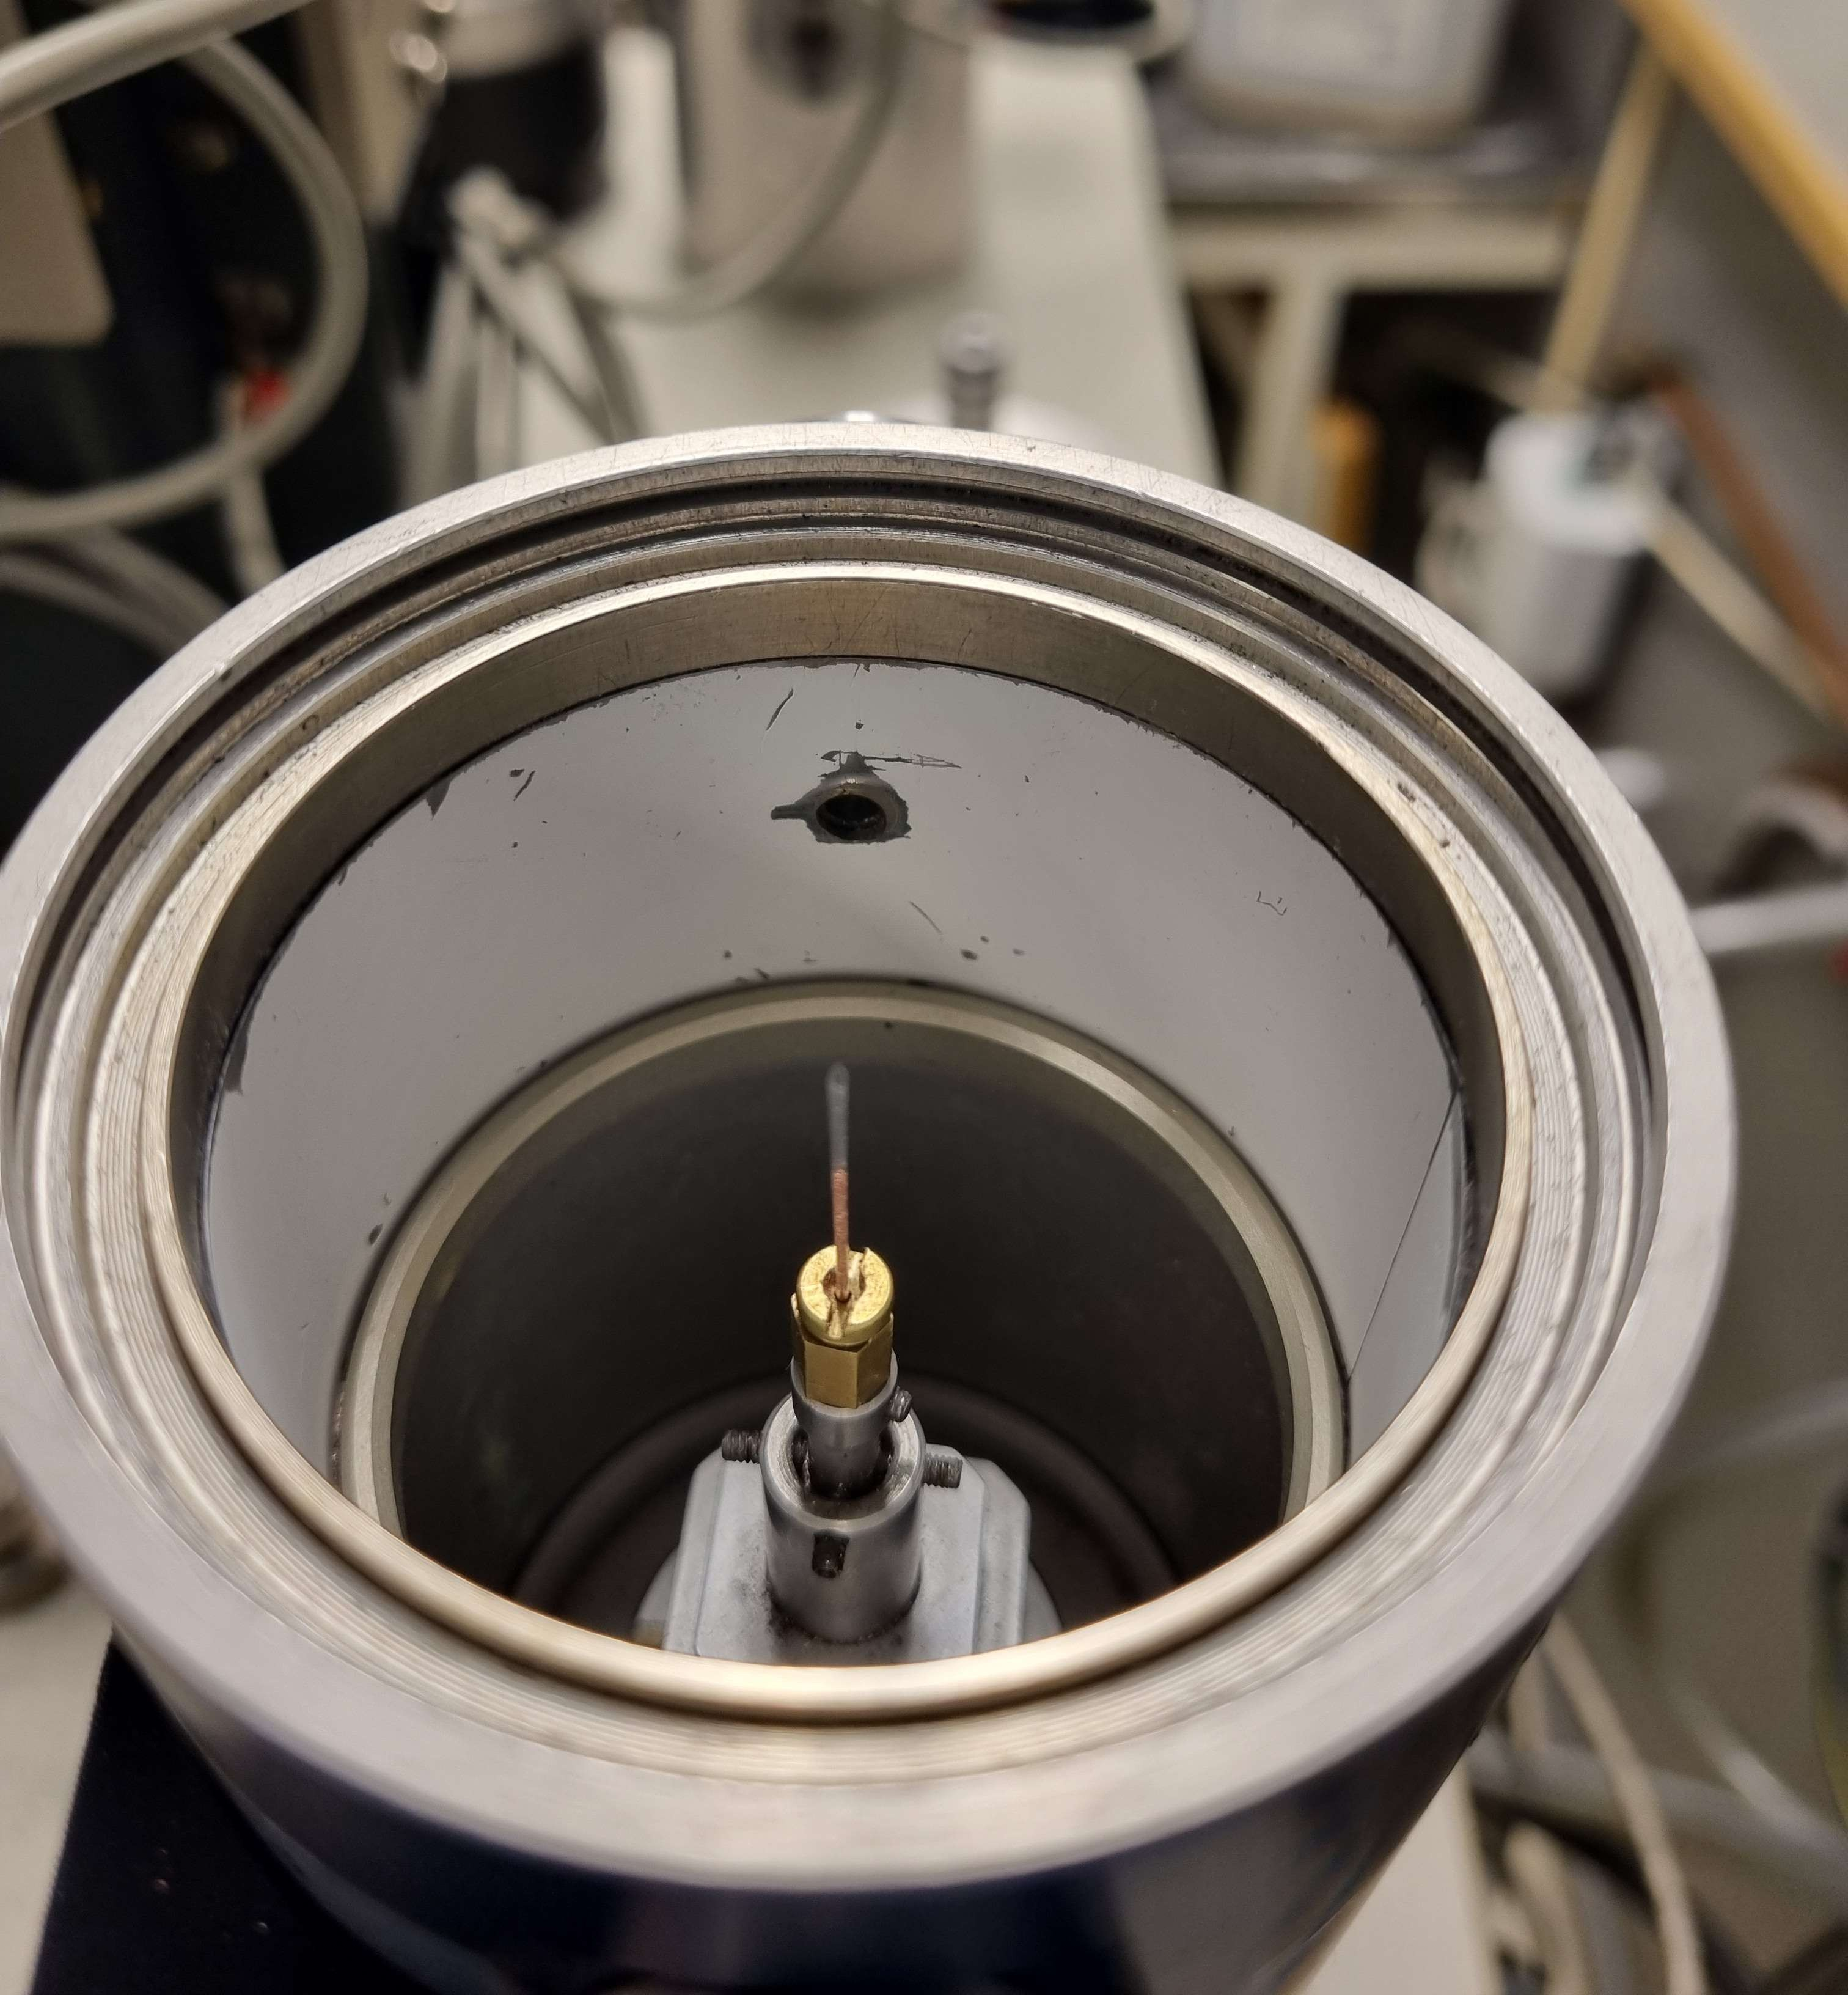
\includegraphics[width=0.33\textwidth]{Bilder/prov i kamera_närbild.jpg}
    \caption{\textit{Debye-Sherrer kamera med monterat kapillärrör som innehåller ett nedfilat, okänt, grundämne. 
    Provet monterades i en hållare som långsamt roterades under hela mätningen.}}
    \label{fig:prov_i_kamera}
\end{figure}

Under 40 minuter bestrålades kapillärröret av röntgenstrålning. Då röret roterades under förloppet erhölls ett diffraktionsmönster bestående av ringar i stället för enskillda punkter.
Röntgenfilmen togs ut och behandlades med fixering och framkallningsvätska innan den hängdes på tork. Efter att filmen torkat togs bilder över ett ljusbord av varje film, ett exempel visas i figur \ref{fig:film2-1}.
Totalt erhölls tre filmer som visade ett diffraktionsmönster.

\begin{figure}[H]
    \centering
    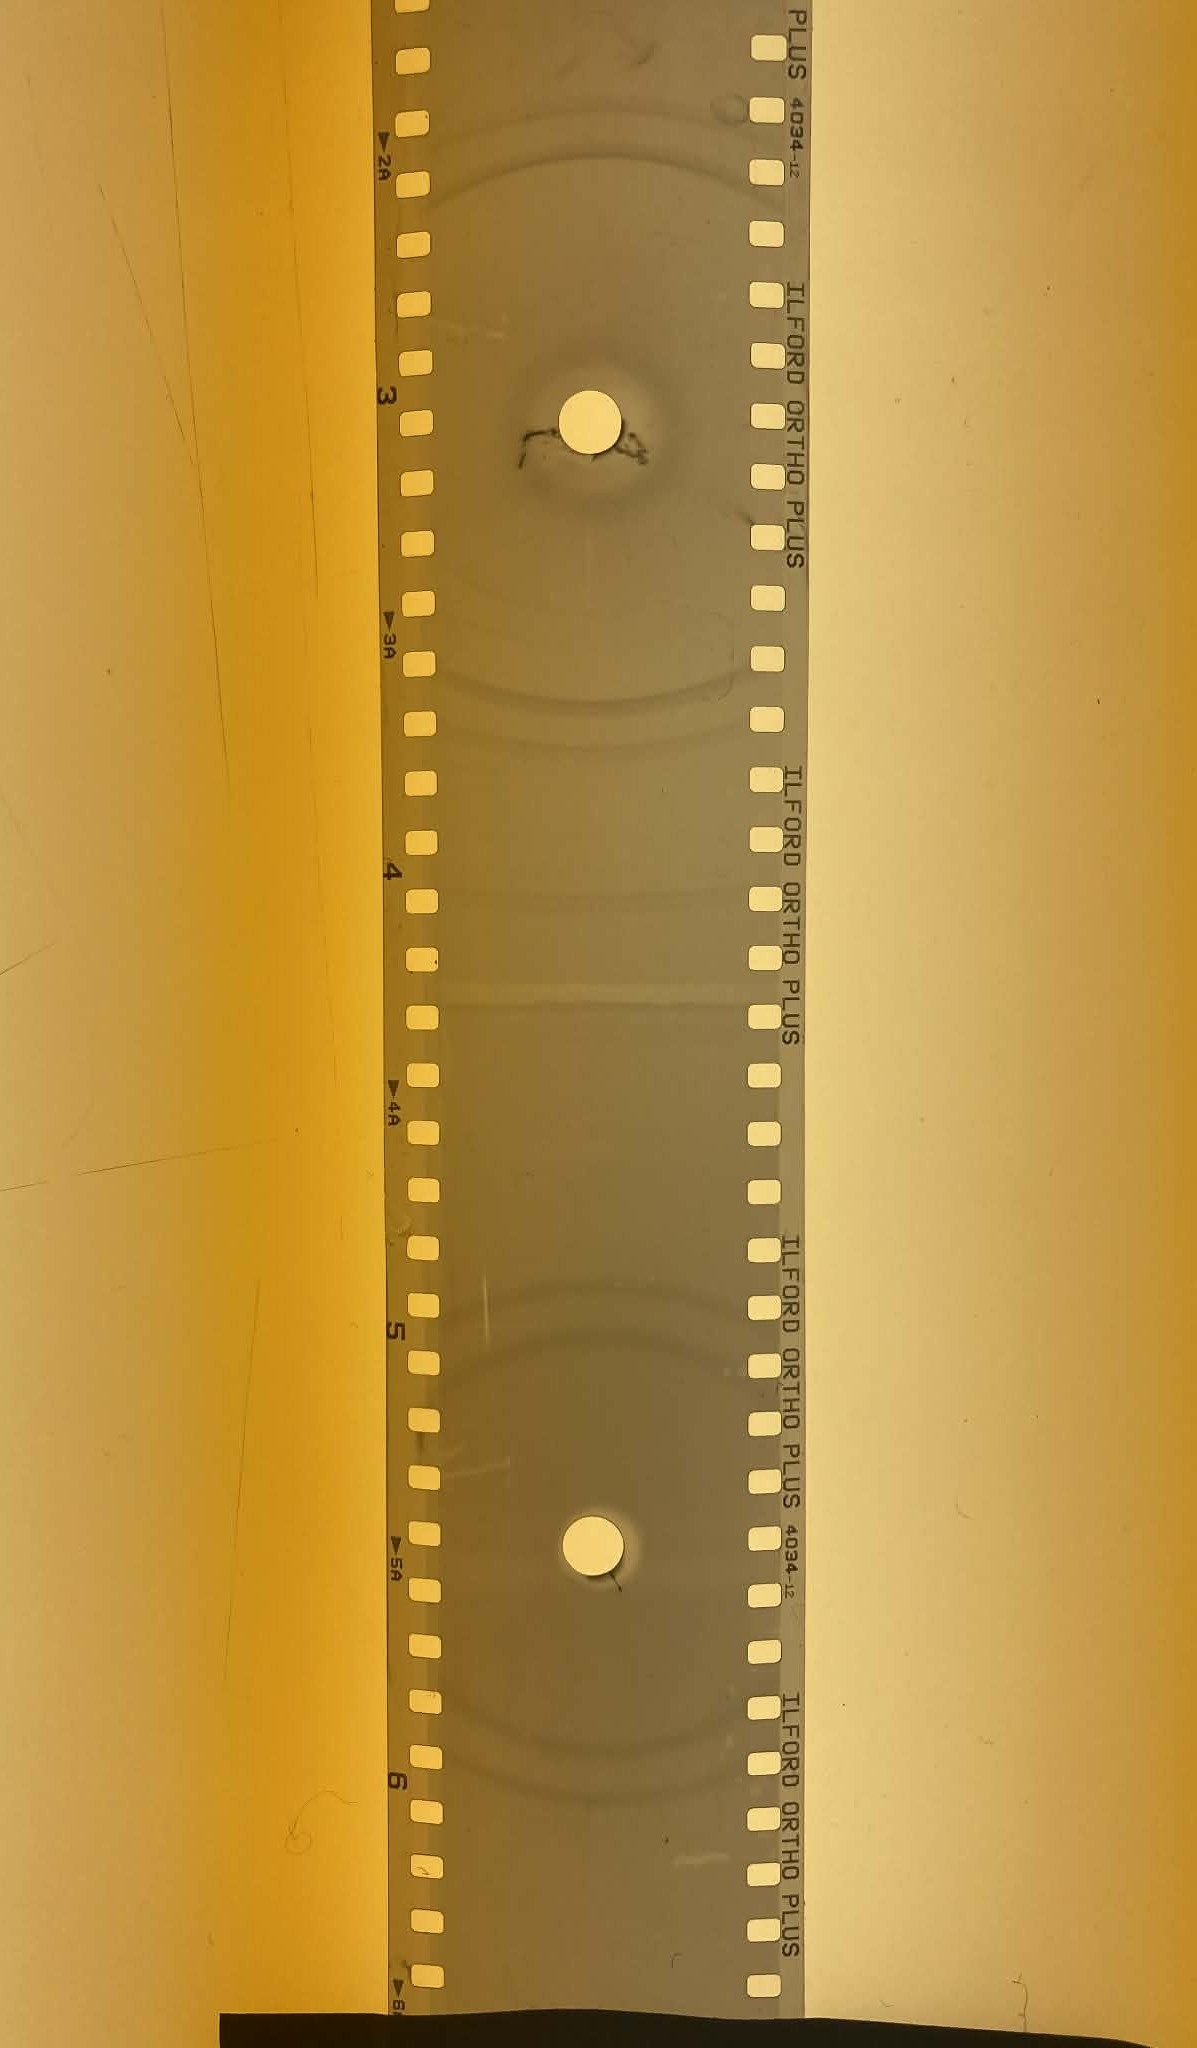
\includegraphics[width=0.33\textwidth, angle=90]{Bilder/film2-1.jpg}
    \caption{\textit{En av tre filmer som erölls under laborationen. På filmen syns flertalet ringar som korresponderar till de reflexer den kristallstruktur det undersökta ämnet tillåter.
    Centrum av röntgenstrålen insträffar i centrum av det vänstra hålet av filmen.}}
    \label{fig:film2-1}
\end{figure}

Därefter bestämdes transmissionsspektrumet för kisel med två olika spektrofotometrar, Cary 5000  och Parkin Elmer 1725. Dessa kan endast mäta vissa våglängdsintervaller, de våglängder som undersöktes valdes däremed för att
maximera det totala spektrumet. I Cary 5000 mättes transmissionsspektrumet över våglängderna 180-3500 nm och med Perkin Elmer mättes intervallet 1500-25000 nm.

\section{Resultat}
Totalt erhölls tre lyckade filmer där diffraktionslinjerna var tydliga nog för mätning. 
Dessa behandlades sedan digitalt för större precision, för full beräkning och kod, se appendix \ref{app:felmarg_gitterparameter} och \ref{app:kod-debye-sherrer}. 
För varje bild hittades de två hålen som filmen fästes i kameran med och en intensitetsfördelning skapades i en linje mellan hålen.
Därefter bildades ett medelvärde av intensitetsfördelningen mellan alla bilder och genom att använda $\texttt{numpy.find\_peaks}$ hittades samtliga
intensitetsbottnar som korresponderar med ringarna på filmen. Den medelvärderade intensitetsfördelningen visas i figur \ref{fig:Intensitetsfördelning}. 
\begin{figure}[H]
    \centering
    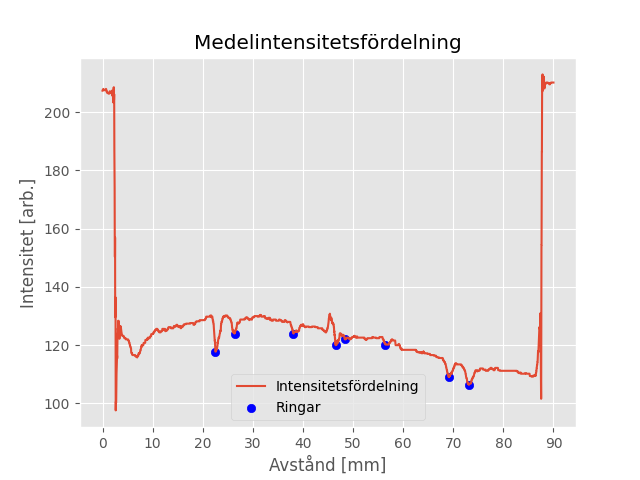
\includegraphics[width=0.75\linewidth]{Bilder/Intensitetsfördelning med bottnar.png}
    \caption{\textit{Den intensitetsfördelning som erhölls genom att medelvärdera intensitetsfördelningen över bilder som togs av kamerafilmerna. I båda kanterna ses hur intensiteten
    snabbt ökar, vilket sker då intensitetfördelningen sträcker sig över de hål som slogs i filmen. I fördelningen hittas flera gropar som representerar de mörka cirklar som erhölls
    på kamerafilmen, dessa gropar markeras även i figuren.}}
    \label{fig:Intensitetsfördelning}
\end{figure}
Från intensitetsfördelningen hittades då avstånden från centrum av det hål där strålcentra sammanfaller och de intensitetsbottnarna där ringarna finns. 
Dessa avstånd visas i tabell \ref{tab:Ringavstånd}.
\begin{table}[H]
    \centering
    \caption{\textit{De avstånd som hittades mellan strålcentra och de markerade groparna i figur \ref{fig:Intensitetsfördelning}. Totalt hittades 8 ringar.}}
    \label{tab:Ringavstånd}
    \begin{tabular}{|c|c|c|c|c|c|c|c|c|}
        \rowcolor{lightgray}
        \hline
        Ring & 1 & 2 & 3 & 4 & 5 & 6 & 7 & 8 \\ \hline
        Avstånd från strålcentra [mm] & 22,9 & 26,3 & 38,7 & 46,9 & 48,6 & 57,0 & 70,0 & 73,9 \\ \hline
    \end{tabular}
    
\end{table}
Från avstånden i tabell \ref{tab:Ringavstånd} kunde sedan en talserie bildas genom att applicera ekvation \ref{Eq:theta från cirkel} och \ref{Eq: Heltalsserie}. Värdena på 
$\lambda$ och $R$ var givna som $\lambda = 1,542$ Å och $2R = 57,8$ cm. Serien normerades med det sista talet och förlängdes för att erhålla en serie som ideelt är en heltalsserie. Den serie som erhölls var

\begin{equation}
    3,28; \ 4,24; \ 8,48; \ 11,55; \ 12,20; \ 15,22; \ 19,13; \ 20,0,
\end{equation}
vilket matchar de reflexer som förväntas finnas i en FCC struktur. Gitterparametern beräknades sedan genom att betrakta \ref{Eq: Heltalsserie} som en linjär relation 
mellan $\sin^2\theta$ och $(h^2+k^2+l^2)$. Linjär regression utfördes och lutningen, som motsvarar konstanten $(\lambda/2a)^2$, bestämdes. För utförligare beräkning av felmarginal, 
se appendix \ref{app:felmarg_gitterparameter}. Från detta kunde sedan gitterparametern bestämmas till
\begin{equation}
    a = 3,611 \pm 0,022 \text{ Å},
\end{equation}
vilket matchar redan känt värde och struktur för koppar.

Därefter bestämdes transmissionsspektrumet för kisel med två spektrometrar, Parkin Elmer och Cary 5000. För båda maskinerna erhölls 5 transmissionsspektrum som sedan medelvärderades
och visas tillsammans med dess medelfel i figur \ref{fig:Transmissionsspektrum}. 

\begin{figure}[H]
    \centering
    \begin{subfigure}{0.49\textwidth}
        \centering
        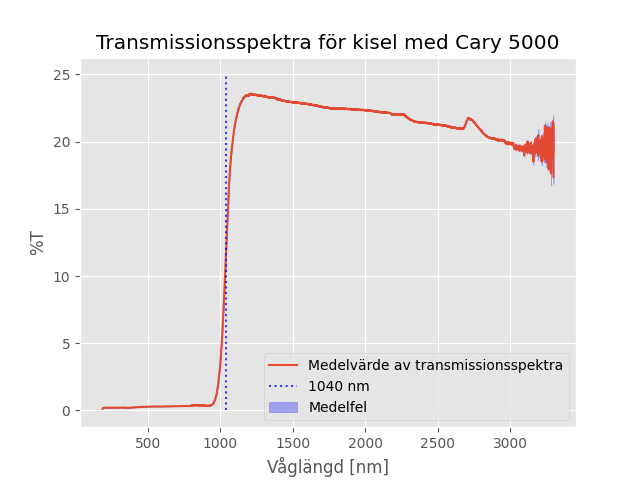
\includegraphics[width=\linewidth]{Bilder/Transmissionsspektra Medel Cary 5000.png}
        \caption{\textit{Transmissionsspektrum från Cary 5000.}}
        \label{fig:transmissionsspektrum_a}
    \end{subfigure}
    \hfill
    \begin{subfigure}{0.49\textwidth}
        \centering
        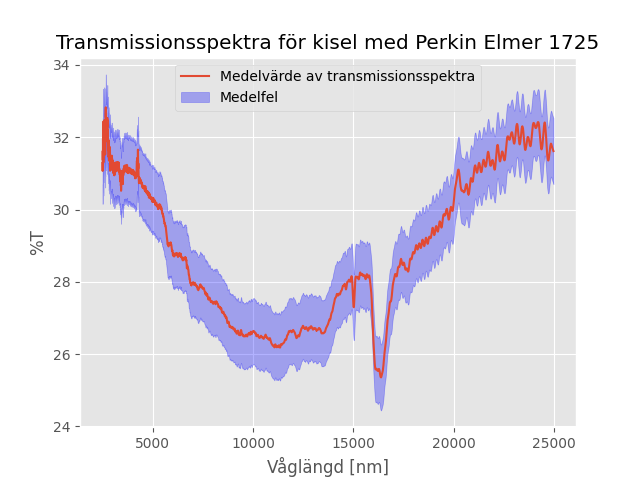
\includegraphics[width=\linewidth]{Bilder/Transmissionsspektra Medel Perkin Elmer 1725.png}
        \caption{\textit{Transmissionsspektrum från Perkin Elmer.}}
        \label{fig:transmissionsspektrum_b}
    \end{subfigure}
    \caption{\textit{Medelvärderade transmissionsspektrum från två olika spektrometrar, Cary 5000 (a) och Perkin Elmer (b). I båda figurerna illustreras även medelfelet som ett intervall
     runt spektrat, vilket visar att medelfelet är ordningsmässigt störrre i mätningarna som utfördes med Perkin Elmer.}}
    \label{fig:Transmissionsspektrum}
\end{figure}

I figur \ref{fig:transmissionsspektrum_a} syns ett abruppt avbrott i transmissionsförmågan. Medelpunkten på detta avbrått estimeras till $1040$ nm, vilket motsvarar energin $1,19$ eV.

\section{Diskussion}
Syftet med laborationen var att inledningsvis identifiera ett för oss okänt grundämne med hjälp av röntgendiffraktion.
Detta gjordes genom att analysera diffraktionsmönstret och därmed bestämma vilka reflexer som avbildades på filmen. 
Genom att jämföra de uppmätta reflexerna med kända serier för olika kristallstrukturer kunde grundämnets kristallstruktur bestämmas till FCC 
och dess gitterparameter till ca 3,61 Å.
Allt sammantaget kunde alltså grundämnet bestämmas som koppar, vilket har en FCC-struktur och en känd gitterparameter på 3,61 Å.

Resultatet är dock osäkert, eftersom den uppmätta heltalsserien för vissa reflexer avviker ganska signifikant från det teoretiska värdet.
För till exempel reflex 6 skall det teoretiska värdet i heltalsserien vara 16, men det beräknade värdet är närmare 15.
Detsamma gäller för reflex 4, som teoretiskt sett borde vara 11 men det beräknade värdet är tydligt närmare 12.
Dessa diskrepanser hade kunnat elimineras om fler mätningar hade genomförts.
Dessa beräkningar är baserade på endast 3 mätningar, vilket får ses som för lite för att kunna uppnå ett tillförlitligt resultat.
Anledningen till detta är den stora andelen misslyckade mätningar samt begränsad tillgång till röntgenkameran.
Av 8 försök ledde 3 till mätbara resultat.

Gitterparametern kunde dock bestämmas med ganska god precision, eftersom linjär regression kunde utföras.
Det beräknade värdet ligger mycket nära det tabulerade värdet för koppar och får därför ses som ett gott resultat.
Den relativt låga felmarginalen bidrar även den till resultatets tillförlitlighet.

Vad gäller transmissionsspektrumet kan man inledningsvis konstatera att där de två spektrofotometrarna överlappar, 
dvs vid en våglängd på ca 3000 nm, skiljer transmissionen mellan dem med ca 10 procentenheter.
Detta får ses komma från olika kalibreringar av maskinerna och kan bortses från fortsättningsvis.

Vad gäller transmissionen för korta våglängder som samlades in från Cary 5000 kan man observera ett tydligt avbrott med en mittpunkt vid ca 1040 nm i figur \ref{fig:Transmissionsspektrum}.
Detta motsvarar en fotonenergi på ca 1,19 eV, vilket är mycket nära kisels bandgap på 1,12 eV.
Figur \ref{fig:transmissionsspektrum_a} visar även att övergången inte är diskret, utan sker i ett område mellan 1000 - 1100 nm.
Anledningen till detta är att i det området kan en foton excitera en elektron samtidigt som den exciterar eller annihilerar en fonon.
Eftersom fononerna är beroende av vågtalet $k$ kan denna excitation ske över ett kontinuerligt energispektrum,
och detta är anledningen till att övergången sker gradvis och inte abrupt.
Detta innebär att kisel har ett indirekt bandgap och inte ett direkt bandgap.

Excitation av fononer är anledningen till att transmissionsspektrumet som visas i figur \ref{fig:transmissionsspektrum_b}.
Nedgången i transmission kommer från multifononabsorption, där en foton absorberas och ger upphov till en eller flera fononer.
Typiska fononfrekvenser visas i tabell \ref{tab:fononfrekvenser}.
Om en foton skulle excitera en fonon i gren TA$_1$ vid symmetripunkt L och en fonon i gren TO$_2$ vid symmetripunkt X skulle den excitationsenergin som krävs motsvara

\begin{equation}
    E_\gamma = hf_1 + hf_2 = h(3,14 + 14,09) \cdot 10^{12} = 17,23h \cdot 10^{12}.
\end{equation}
Detta motsvarar en fotonvåglängd på 17,4 µm, vilket är exakt det vi ser i figur \ref{fig:transmissionsspektrum_b}.
Transmissionen går alltså ned i våglängdsområdet 5 - 20 µm eftersom fotoner exciterar fononer, 
och fononerna har kvantiserade energier som motsvarar dessa våglängder.
\section{Slutsatser}

Med hjälp av röntgendiffraktion kunde det okända ämnets kristallstruktur bestämmas till en FCC-struktur,
och dess gitterparameter kunde bestämmas till $3,611 \pm 0,022 \; \text{Å}$.
Detta gör att ämnet kunde bestämmas till koppar, 
vars kristallstruktur är känd som FCC och dess gitterparameter är känd som 3,61 Å.
Den resulterade heltalsserien hade avvikelser från den teoretiska heltalsserien.
Detta tros bero på den begränsade mängden mätdata som i sig kom sig av flertalet misslyckade mätningar.
Det resulterande värdet för gitterparametern får dock ses som tillförlitligt på grund av den resulterande låga felmarginalen.

Med hjälp av transmissionsspektrum kunde bandgapet för kisel bestämmas till ca 1,19 eV, vilket är nära det tabulerade värdet på 1,12 eV.
Eftersom transmissionsspektrumet inte betedde sig som en stegfunktion vid bandgapet utan uppvisade ett mer gradvis avtagande av transmissionen 
kunde slutsatsen dras att kisel har ett indirekt bandgap och inte ett direkt bandgap.

Nedgången i transmission som observeras i våglängdsområdet 5 - 20 µm beror på multifononabsorption, 
där fotoner det våglängdsområdet exciterar en eller flera fononer.

\newpage

\printbibliography

\newpage

\appendix
\section{Beräkning av felmarginal för gitterparameter}
\label{app:felmarg_gitterparameter}
Gitterparametern beräknades genom att utföra viktad linjär regression på uttrycket
\begin{equation}
    4\sin^2(\theta) = \left(\dfrac \lambda a\right)^2 (h^2+k^2+l^2)
\end{equation}
som kan betraktas som en linjär funktion enligt
\begin{equation}
    y = k x + m,
\end{equation}
där $y = 4\sin^2(\theta)$ och $x = (h^2+k^2+l^2)$. För detta användes $\texttt{numpy.polyfit}$ där konstanterna $k = \left(\dfrac \lambda a\right)^2$ och $m$ anpassades 
med minsta kvadratmetoden. De erhållna värdena viktades med vikterna $1/\sigma^2_{y}$, där $\sigma_{y}$ erhölls genom felfortplantning enligt 
\begin{equation}
    \sigma_y = 8\sin\theta \cos\theta \sigma_\theta,
\end{equation}
där $\sigma_\theta$ är osäkerheten i vinklarna $\theta$ som på liknande sätt erhålls via felfortplantning enligt
\begin{equation}
    \sigma_\theta = \dfrac{\sigma_{tot}}{2R},
\end{equation}
där $R$ är kameraradien $28,9$ cm och $\sigma_{tot}$ är den totala standardavvikelsen i de avstånd som presenteras i tabell \ref{tab:Ringavstånd}. Den totala standardavvikelsen beror både
på den statistiska spridningen i mätningarna, $\sigma_r$, och det diskretiseringsfel som uppkommer från pixelisering av filmerna, $\sigma_{kod}$. Det antogs att de avstånd som hittades i intensitetsfördelningen 
hade osäkerhet av 1 pixel. Den totala osäkerheten blir därmed
\begin{equation}
    \sigma_{tot} = \sqrt{\sigma_r^2 + \sigma^2_{kod}}.
\end{equation} 
Standardavvikelsen i mätningarna erhölls genom att använda $\texttt{numpy.std}$ och ett $95\%$ konfidensintervall beräknades med Student-t-fördelningen enligt
\begin{equation}
    \sigma_r = t_{0,975, n-1}\dfrac{\sigma}{\sqrt{n}},
\end{equation}
där $\sigma$ är standardavvikelsen för ett stickprov och $n$ är antalet mätningar.

Från $\texttt{numpy.polyfit}$ erhålls även kovariansmatrisen för regressionen, och standardavvikelsen för $k$, $\sigma_k$, beräknades genom att ta roten ur dess korresponderande diagaonalelement.
Osäkerheten i gitterparametern, $a$, beräknades sedan med felfortplantning enligt
\begin{equation}
    \sigma_a = \dfrac{\lambda}{2k^{3/2}}\sigma_k,
\end{equation}
där $\lambda$ är den genomsnittliga våglängden på den röntgenstrålning som nyttjades, enligt uppgift gäller $\lambda = 1,542$ Å. Med insatta värden för $R$, $\lambda$ erhålls en felmarginal för $a$ på
\begin{equation}
    0,022 \text{ Å}.
\end{equation}

\section{Kod för data- och felanalys}
Nedan presenteras all kod som användes för att utföra data- och felanalys av både gitterparametern och transmissionsspektrumet.
\subsection{Kod för data- och felanalys av gitterparameter}
\label{app:kod-debye-sherrer}
Nedan presenteras den kod som användes för att analysera kamerafilmerna från Debye-Sherrer-experimentet.
\begin{lstlisting}[style=mypython, label={lst:dataanalys_Debye-Sherrer}]
import cv2
import numpy as np
import matplotlib.pyplot as plt
from scipy.signal import find_peaks
from scipy.ndimage import gaussian_filter1d
from scipy.stats import t
from matplotlib.ticker import MaxNLocator

intensitydist = []

# Läs bilder
img_raw = np.array([
        cv2.imread("dataanalys/Grunduppgift-data/film1-1.jpg"), 
        cv2.imread("dataanalys/Grunduppgift-data/film1-3.jpg"), 
        cv2.imread("dataanalys/Grunduppgift-data/film2-1.jpg"),
        cv2.imread("dataanalys/Grunduppgift-data/film2-2.jpg"), 
        cv2.imread("dataanalys/Grunduppgift-data/film2-3.jpg"),])
for i in range(len(img_raw)):
    # Introducera litet "blur" för att hitta rätt cirklar
    img = cv2.rotate(img_raw[i], cv2.ROTATE_90_COUNTERCLOCKWISE)
    gray = cv2.cvtColor(img, cv2.COLOR_BGR2GRAY)
    gray_blur = cv2.GaussianBlur(gray, (9, 9), 2)

    # Hitta centrum av de två hålen
    circles = cv2.HoughCircles(
        gray_blur,
        cv2.HOUGH_GRADIENT,
        dp=1.2,
        minDist=100,
        param1=50,
        param2=30,
        minRadius=10,
        maxRadius=130
    )

    circles = np.around(circles).astype(int)
    (x11, y11, r11), (x22, y22, r22) = circles[0][:2]
    # Ordna hålen från vänster till höger
    if x11 < x22:
        x1, y1 = x11, y11
        x2, y2 = x22, y22
    else:
        x1, y1 = x22, y22
        x2, y2 = x11, y11

    # Skapa samples längs en linje mellan cirkelcentrum
    samples = 5000
    xs = np.linspace(x1, x2, samples, endpoint=True)
    ys = np.linspace(y1, y2, samples, endpoint=True)
    profile = []

    # Ta en intensitetsfördelning längs den samplade linjen
    for x, y in zip(xs, ys):
        xi, yi = int(round(x)), int(round(y))
        profile.append(gray[yi, xi])

    profile = np.array(profile)
    intensitydist.append(profile)

# Skapa en medelintensitetsfördelning
intensitydist = np.mean(intensitydist, 0)

# Ta bort område innan första ringen (undvika onödiga bottnar)
n = len(intensitydist)

mask = np.ones(n, dtype=bool)

# Sätt marginal
margin = int(0.15 * n)
mask[:margin] = False
mask[-margin:] = False

valid_indices = np.where(mask)[0]
filtered_profile = intensitydist[mask]

# Hitta bottnar i intensitetsfördelningen med find_peaks
inv = - filtered_profile
baseline = gaussian_filter1d(inv, sigma=100)
corrected = inv - baseline
peaks, _ = find_peaks(corrected, distance=190, prominence=2, width=1, plateau_size=1)

# Manuellt lägg till 12-toppen där den "ska vara"
range12 = [peaks[3]+100, peaks[4]-100]
peak12 = np.where(corrected == np.max(corrected[range12[0]:range12[1]]))[0][0]
peaks = np.insert(peaks, 4, peak12)
peaks = valid_indices[peaks]


# Skala om till verklig längd
# Pixelavstånd mellan hålen
pixel_dist = np.sqrt((x2 - x1)**2 + (y2 - y1)**2)
meter_per_pixel = 0.09 / pixel_dist

# Hitta peaks i varje bild givet att vi vet ungefär vart de ska vara
window = 50
all_vals = []

for i in range(len(img_raw)-1):
    img = cv2.rotate(img_raw[i], cv2.ROTATE_90_COUNTERCLOCKWISE)
    gray = cv2.cvtColor(img, cv2.COLOR_BGR2GRAY)
    gray_blur = cv2.GaussianBlur(gray, (9, 9), 2)

    circles = cv2.HoughCircles(
        gray_blur,
        cv2.HOUGH_GRADIENT,
        dp=1.2,
        minDist=100,
        param1=50,
        param2=30,
        minRadius=10,
        maxRadius=130
    )

    circles = np.around(circles).astype(int)
    (x11, y11, r11), (x22, y22, r22) = circles[0][:2]

    if x11 < x22:
        x1, y1 = x11, y11
        x2, y2 = x22, y22
        r1 = r11
        r2 = r22
    else:
        x1, y1 = x22, y22
        x2, y2 = x11, y11
        r1 = r22
        r2 = r11

    xs = np.linspace(x1, x2, samples, endpoint=True)
    ys = np.linspace(y1, y2, samples, endpoint=True)

    profile = []
    for x, y in zip(xs, ys):
        xi, yi = int(round(x)), int(round(y))
        profile.append(gray[yi, xi])

    profile = np.array(profile)
    vals = []

    # I ett fönter runt varje medelpeak, hitta minimum för aktuell bild
    for p in peaks:
        left = max(0, p - window)
        right = min(len(profile), p + window)

        local_idx = np.argmin(profile[left:right])
        true_idx = left + local_idx

        px = xs[true_idx]
        py = ys[true_idx]

        dist_pixels = np.sqrt((px - x1)**2 + (py - y1)**2)
        dist_m = dist_pixels * meter_per_pixel

        vals.append(dist_m)

    all_vals.append(vals)

    output = img.copy()


    # # Rita på bilden vart ringarna finns, för debugging
    # # Rita linje
    # cv2.line(output, (x1, y1), (x2, y2), (255, 0, 0), 2)
    # cv2.circle(output, (x1, y1), 10, (255,0,0), r1)
    # cv2.circle(output, (x2, y2), 10, (0,255,0), r2)

    # # Rita detekterade punkter
    # for p in peaks:
    #     px = int(xs[p])
    #     py = int(ys[p])
    #     cv2.circle(output, (px, py), 3, (0, 0, 255), -1)

    # cv2.namedWindow("Line detection", cv2.WINDOW_NORMAL)
    # cv2.imshow("Line detection", output)
    # cv2.waitKey(0)
    # cv2.destroyAllWindows()

# Alla peakavstånd i alla bilder
all_vals = np.array(all_vals)

# Beräkna standardavvikelsen för peakavstånden
n = all_vals.shape[0]

mean_vals = np.mean(all_vals, axis=0)
std_vals = np.std(all_vals, axis=0, ddof=1)

# Ta 95% konfidensintervall
tval = t.ppf(0.975, n-1)

# instrumentfel
sigma_pixel = 1
sigma_instr = meter_per_pixel * sigma_pixel

total_std = np.sqrt(std_vals**2 + sigma_instr**2)

sigma_vals = tval * total_std / np.sqrt(n)

vals = mean_vals

print("Vals (mm):", 1000 * vals)
print("Osäkerhet (mm):", 1000 * sigma_vals)

# Visa plot över intensitetsfördelningen
distances_mm = np.linspace(0, 90, samples)
plt.style.use('ggplot')
fig, ax = plt.subplots()
plt.plot(distances_mm, intensitydist, label = 'Intensitetsfördelning')
plt.scatter(distances_mm[peaks], intensitydist[peaks], color='blue', label = 'Ringar')
plt.xlabel('Avstånd [mm]')
plt.ylabel('Intensitet [arb.]')
plt.title("Medelintensitetsfördelning")
ax.xaxis.set_major_locator(MaxNLocator(nbins=10))  # increase tick count
plt.legend()
plt.savefig('Intensitetsfördelning med bottnar.png')


# Manuellt mätta avstånd för de tre filmerna
# vals1 = np.array([22, 25.5, 37.5, 46, 47.8, 69, 73])/1000
# vals2 = np.array([22.1,26,36.6,45.6,47.4,68.7,73])/1000
# vals3 = np.array([22.1,25.8,37.7,45,47.8,68.5,72.8])/1000

# Kod för att få fram heltalsserie, gitterparameter och osäkerheter
R = (57.3/2)/1000
lam = 1.542e-10

theta = vals / (2 * R)
sigma_theta = np.sqrt((sigma_vals / (2 * R))**2)

series = 4 * np.sin(theta)**2 / lam**2
sigma_series = (8 * np.sin(theta) * np.cos(theta) / lam**2) * sigma_theta

series0 = series[-1]
sigma_series0 = sigma_series[-1]

series_norm = 20*series/series0
sigma_series_norm = series_norm * np.sqrt((sigma_series / series)**2 + (sigma_series0 / series0)**2)

hkl_real = np.array([3,4,8,11,12,16,19,20])
y = 4 * np.sin(theta)**2
weights = 1/(sigma_series**2)

coeffs, cov = np.polyfit(hkl_real, y, 1, w=weights, cov = True)
slope = coeffs[0] # y = (lambda/a)**2 x
sigma_slope = np.sqrt(cov[0,0])

a = lam/np.sqrt(slope)
sigma_a = (lam / (2*slope**(1.5)))*sigma_slope

print("Heltalserie:", ", ".join(f"{val:.2f} ± {err:.2f}" for val, err in zip(series_norm, sigma_series_norm)))
print(f"a = {(a/1e-10):.4} ± {(sigma_a/1e-10):.2} Å")
\end{lstlisting}


\subsection{Kod för data- och felanalys av transmissionsspektrum}
\label{app:kod-transmission}
Nedan presenteras den kod som användes för att analysera datan från Cary 5000 och Perkin Elmer 1725.
\begin{lstlisting}[style=mypython, label={lst:dataanalys_transmission}]
import numpy as np
import matplotlib.pyplot as plt
import pandas as pd

plt.style.use('ggplot')

# -- Mätning med Cary 5000 --
# Ta in data
data_CARY = pd.read_csv('dataanalys/Spektroskopi-data/Transmission_kisel_OFFICIELL.csv', skiprows=1, skipfooter=194, engine='python')
data_CARY = data_CARY.dropna(axis=1, how="all")
datasets_CARY = []

for i in range(0, len(data_CARY.columns), 2):
    sub = data_CARY.iloc[:, i:i+2].copy()
    sub.columns = ['Wavelength (nm)', '%T']
    sub = sub.dropna()
    datasets_CARY.append(sub)

baseline = datasets_CARY[0]
wavelengths_CARY = baseline['Wavelength (nm)']
samples = datasets_CARY[1:]

# Medelvärdera, plotta och ta fram standardavvikelse
T_values_CARY = 100*np.array([s["%T"].values for s in samples]) / np.array([baseline["%T"].values])
T_mean_CARY = np.mean(T_values_CARY, axis=0)
T_std_CARY = np.std(T_values_CARY, axis=0)
T_SEM_CARY = T_std_CARY / np.sqrt(len(samples))

fig, ax = plt.subplots()
plt.plot(wavelengths_CARY, T_mean_CARY, label = 'Medelvärde av transmissionsspektra')
plt.fill_between(wavelengths_CARY, T_mean_CARY - T_SEM_CARY, T_mean_CARY + T_SEM_CARY, alpha=0.3, color = 'b', label="Medelfel")
plt.xlabel("Våglängd [nm]")
plt.ylabel("%T")
plt.title('Transmissionsspektra för kisel med Cary 5000')
plt.legend()
plt.savefig('Transmissionsspektra Medel Cary 5000')


# -- Mätning med PerkinElmer --
# Ta in data
datasets_PE = [pd.read_csv('dataanalys/Spektroskopi-data/student 07.csv', sep=";", encoding='latin1', skiprows=1, decimal=","),
        pd.read_csv('dataanalys/Spektroskopi-data/student 09.csv', sep=";", encoding='latin1', skiprows=1, decimal=","),
        pd.read_csv('dataanalys/Spektroskopi-data/student 10_1.csv', sep=";", encoding='latin1', skiprows=1, decimal=","),
        pd.read_csv('dataanalys/Spektroskopi-data/student 11.csv', sep=";", encoding='latin1', skiprows=1, decimal=","),
        pd.read_csv('dataanalys/Spektroskopi-data/student 13.csv', sep=";", encoding='latin1', skiprows=1, decimal=",")]


# Medelvärdera, plotta och ta fram standardavvikelse
wavelengths_PE = datasets_PE[0]['nm']
wavelengths_PE = wavelengths_PE[268:]
T_values_PE = np.array([s['%T'].values for s in datasets_PE])
T_values_PE = T_values_PE[:, 268:]

# Troubleshooting plot
# for i in range(len(T_values_PE)):
#     plt.plot(wavelengths_PE, T_values_PE[i])
#     plt.show()

T_mean_PE = np.mean(T_values_PE, axis=0)
T_std_PE = np.std(T_values_PE)
T_SEM_PE = T_std_PE/np.sqrt(len(datasets_PE))

fig, ax = plt.subplots()
plt.plot(wavelengths_PE, T_mean_PE, label = 'Medelvärde av transmissionsspektra')
plt.fill_between(wavelengths_PE, T_mean_PE - T_SEM_PE, T_mean_PE + T_SEM_PE, alpha=0.3, color = 'b', label="Medelfel")
plt.xlabel("Våglängd [nm]")
plt.ylabel("%T")
plt.title('Transmissionsspektra för kisel med Perkin Elmer 1725')
plt.legend()
plt.savefig('Transmissionsspektra Medel Perkin Elmer 1725')


\end{lstlisting}

\section{Labblogg}
Nedan presenteras den labblogg som skrevs under laborationen.
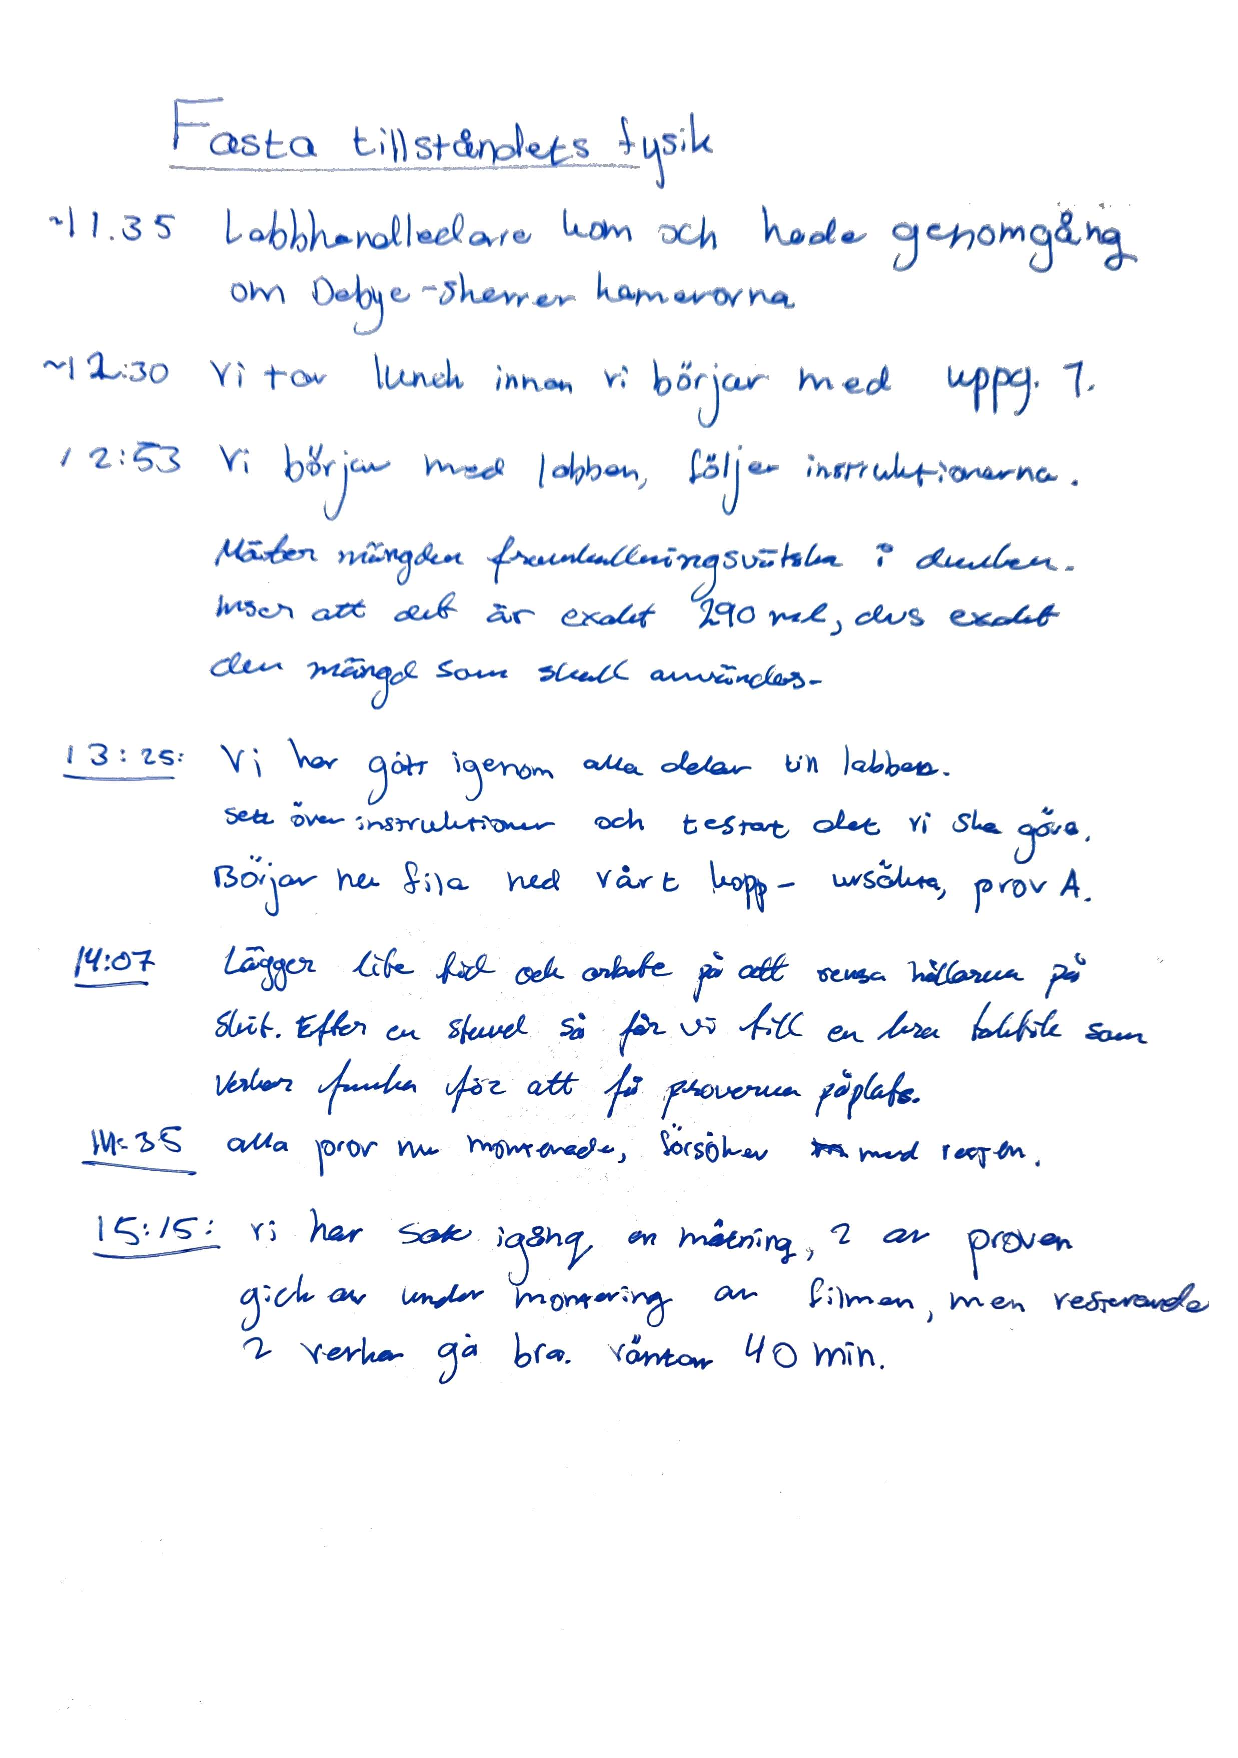
\includepdf[pages=-]{Labblogg Fasta Tillståndets Fysik.pdf}

\end{document}
